Studiamo adesso in dettaglio il legame chimico.

Prima di addentrarci nell'argomento però, bisogna notare che esistono speci chimiche di cui non esiste la molecola, ma solo il solido: i composti ionici. Un esempio di tali composti è l'NaCl: la specie molecolare del cloruro di sodio non esiste, ma esiste il solido.

Dobbiamo allora comprendere perché non esistano le molecole singole delle speci fortementi ioniche, per poi ragionare sul legame chimico, che ha una natura diversa nei sistemi molecolari.

Dobbiamo quindi rispondere a una serie di domande:
\begin{itemize}
    \item Perché si formano le molecole, dato che molti sistemi non esistono come tali?
    \item Quali condizioni bisogna soddisfare affinché il composto che si forma a seguito di una reazione, sia stabile?
    \item Perché esistono geometrie ben definite?
\end{itemize}
Prima di andare avanti va da ricordare che in linea generale se facciamo reagire una specie A con una specie B otterremo una specie C in modo spontaneo solo se l'energia del sistema diminuisce. 

Ricordiamo poi che qualunque stato legato avrà un'energia potenziale negativa: in un sistema AB dove A e B sono due atomi, essi sono legati se la loro energia potenziale è minore di zero. Se per qualche motivo l'energia dovesse aumentare, nell'istante in cui essa diventasse pari a zero gli atomi non sarebbero più legati.

Ragioniamo solo sull'energia potenziale per via dell'esistenza del teorema del viriale, il quale afferma che

"\textit{La variazione dell'energia totale di un sistema ha lo stesso segno della variazione dell'energia potenziale}"

Quindi la molecola AB si formerà nel momento in cui l'energia potenziale dei due atomi A e B diminuisce (fino a diventare negativa) man mano che li avviciniamo.\\

Per una molecola o un sistema di pochi atomi siamo in grado di fare ragionamenti estremamente sofisticati anche se non riusciamo a risolvere con esattezza l'equazione di Schrödinger ma solo in maniera ragionevolmente approssimata, nel senso che le soluzioni ottenute non si discotano molto da valori che si ottengono sperimentalmente, ossia la descrizione approssimata risulta essere estremamente accurata per le capacità di calcolo e di modellizzazione ad oggi a disposizione.

Per essi si usa la teoria degli orbitali molecolari, che vedremo dopo.

Nell'istante in cui invece i sistemi che indaghiamo diventano complessi (molti atomi, molecole grandi con elevati pesi molecolari), non siamo più in grado, solo per esigenze di calcolo, di ottenere soluzioni approssimate ragionevolmente

Per essi allora bisogna usare una catalogazione precedente, che si basava sul tipo di legame presente tra le molecole in esame.
Un parametro estremamente utile a comprendere i sistemi è il concetto di elettronegatività, che è la tendenza che hanno i diversi atomi ad attrarre su di sé la carica di legame. Nel momento in cui uno dei due atomi costituenti il nucleo è abbastanza più elettronegativo dell'altro, si avrà una dislocazione della carica di legame, per cui diremo che la molecola avrà una sua polarità, ossia mostrerà una parziale carica positiva e una parziale carica negativa, la quale nei fatti costituisce un dipolo.

In base al valore della differenza di elettronegatività, il legame verrà etichettato in vari modi:
\begin{itemize}
    \item Se è piccola (fino a 0.4) si parla di \textbf{legame covalente};
    \item Se inizia a crescere ma è comunque contenuta (da 0.4 fino a 1.9) si parla di \textbf{legame} covalente \textbf{polare}, e la molecola avrà una polarità cospicua. 
    \item Se diventa molto grande (da 1.9 in poi) si parla di \textbf{legame ionico}.
\end{itemize} 

\subsection{Il legame polare}
In questo caso ci saranno parziali cariche positive e negative, che possono venire indicate in diversi modi: o rispettivamente con $\delta^+$ e $\delta^-$, o con zone rosse e blu che indicano rispettivamente addensamento di elettroni e le zone che si sono positivizzate, o con una freccia con la punta e una croce, dove la punta è rivolta verso l'atomo più elettronegativo.

\subsection{Il legame metallico}
È necessario fare un discorso a parte per i sistemi metallici. Per essi è possibile immaginare che gli elettroni siano abbastanza liberi, nel senso che rispetto ai legami visti in precedenza gli elettroni sono legati pochissimo all'atomo, tanto da essere considerati come un gas che statisticamente neutralizza i nuclei, il quale viene detto "mare di elettroni".

\begin{figure}[htp]
    \centering
    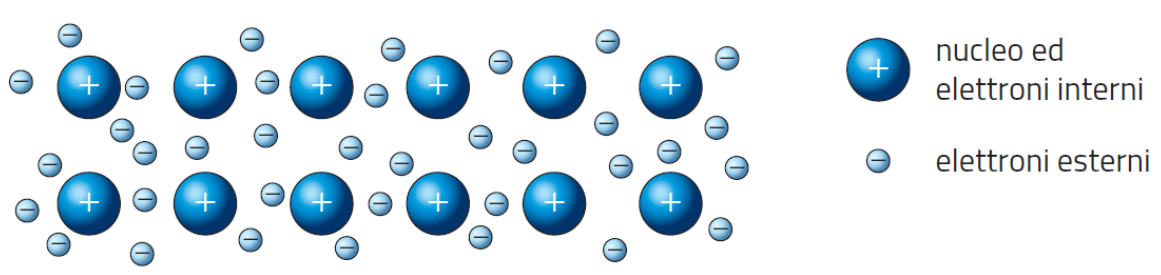
\includegraphics[width=12cm]{immagini/legame-metallico.png}
\end{figure}

Nei metalli gli atomi occupano posizioni ben definite all'interno di una struttura cristallina. A differenza dei composti ionici però qua non possiamo parlare di ioni: gli atomi sono neutri, solo che i loro elettroni esterni occupano una banda e non più un livello. Finora infatti abbiamo parlato di energie ben precise per gli orbitali, ma non è più così all'interno di una banda, o per meglio dire l'energia dei singoli livelli continua ad esserci, ma poiché essi sono in numero elevato, possiamo immaginare che la differenza in energia tra un livello energetico e il successivo sia piccolissima, al punto tale da immaginare non più l'esistenza di orbitali con energie nette e separate, ma una banda all'interno della quale l'elettrone possa muoversi

\subsection{Esempi vari}
Nei vari esempi che seguono, per razionalizzare i i valori sperimentali dei momenti di dipolo, ragioneremo sulla direzionalità dei legami e sulla differenza di elettronegatività degli atomi coinvolti.

\vspace{0.2cm}$\bullet$ ES1 F$_2$

\begin{figure}[htp]
    \centering
    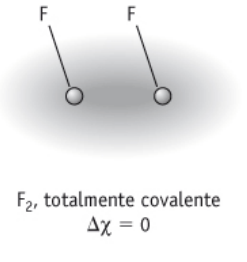
\includegraphics[width=4cm]{immagini/F_2.png}
\end{figure}

Due atomi di fluoro formano la molecola F$_2$. Sebbene il fluoro sia estremamente negativo, i due atomi sono uguali, per cui la differenza in elettronegatività è pari a zero, quindi la condivisione dei due elettroni di legame è totale e il sistema è covalente.

\vspace{0.2cm}$\bullet$ ES2 HF

\begin{figure}[htp]
    \centering
    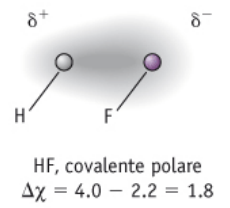
\includegraphics[width=5cm]{immagini/HF.png}
\end{figure}
Nell'acido fluoridrico la differenza di elettronegatività tra i due atomi è cospicua, e infatti la carica di legame(che può essere immaginata come una nube elettronica che circonda i due atomi) sarà più spostata verso l'atomo di fluoro e quindi meno presente sull'idrogeno. Il legame sarà allora covalente polare, con una parziale carica negativa $\delta^-$ sul fluoro e una parziale carica positiva $\delta^+$ sull'idrogeno. 

\vspace{0.2cm}$\bullet$ ES3 LiF

\begin{figure}[htp]
    \centering
    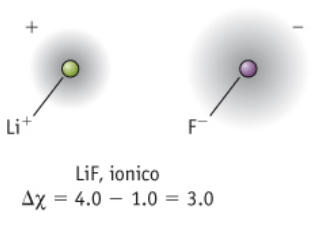
\includegraphics[width=5cm]{immagini/LiF.png}
\end{figure}

In un sistema come il fluoruro di litio, la differenza di elettronegatività è elevata, per cui non ci sarà la nube continua tra i due atomi.

Per questi sistemi si immagina che si abbia una cessione di elettroni, per cui non avremo Li e F ma Li$^+$ e F$^-$, cioè è come se il litio avesse ceduto il suo elettrone di valenza al fluoro, il quale tralaltro acquistandolo avrà la configurazione elettronica esterna dei gas nobili.
Un sistema siffatto è etichettato sistema ionico.

\vspace{0.2cm}$\bullet$ ES4 HCl

\begin{figure}[htp]
    \centering
    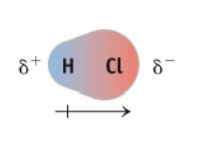
\includegraphics[width=5cm]{immagini/HCl.png}
\end{figure}

Nell'acido cloridrico la differenza di elettronegatività tra idrogeno e cloro è abbastanza evidente, per cui il legame è covalente polare.

Dato che stiamo ipotizzando che su tale molecola ci sia una buona polarità, come conseguenza ci aspettiamo un momento di dipolo.
Per verificarne l'esistenza basta mettere dell'HCl gassoso in un contenitore dove presenti le espansioni polari di un elettromagnete. Se il campo elettrico è nullo, l'orientazione delle molecole sarà casuale; se invece applichiamo una differenza di potenziale tra le due piastre osserveremo che le molecole si orientano in modo tale che il cloro sia rivolto verso la lamina positiva (a potenziale maggiore).
\begin{figure}[htp]
    \centering
    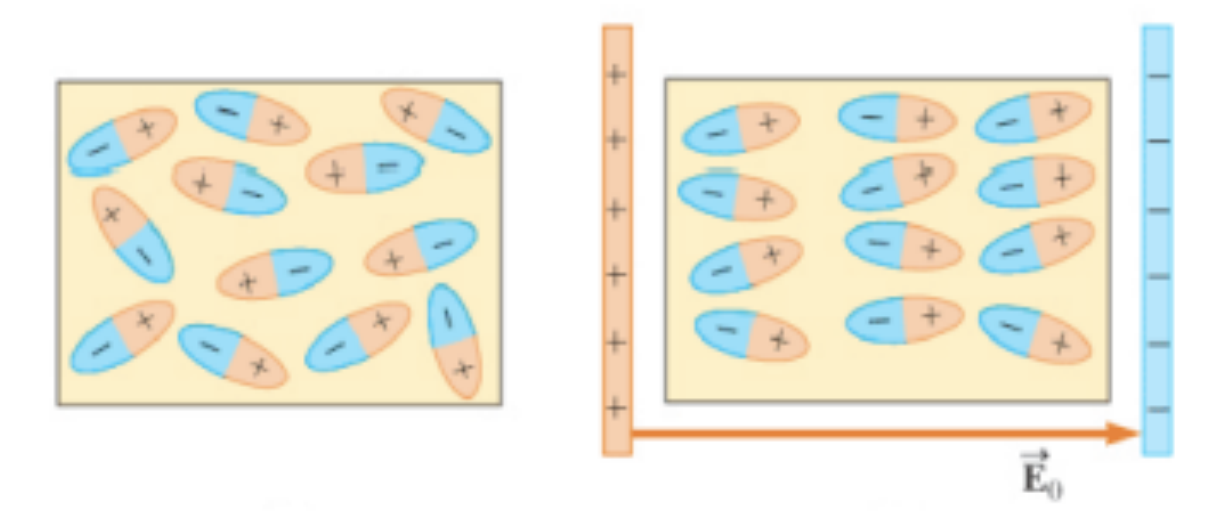
\includegraphics[width=10cm]{immagini/condensatore.png}
\end{figure}
Come facciamo ad accorgercene?
Il sistema che si viene così a costituire è un condensatore, dove tra le armature anziché il vuoto c'è un dielettrico: l'HCl. In questo modo possiamo quindi misurare il momento di dipolo, la cui unità di misura nel SI è il Coulomb per metro, con cui le molecole danno dei valori dell'ordine di 10$^{-30}$, per cui si una un'altra unità di misura che è il Debye (D). Vale la relazione:
$$1D=3.336\cdot10^{-30}$$
Per l'acido cloridrico si misura un momento di dipolo pari a 1.03 D.

\vspace{0.2cm}$\bullet$ ES5 CO$_2$

\begin{figure}[htp]
    \centering
    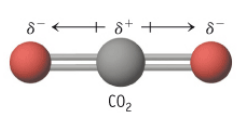
\includegraphics[width=4cm]{immagini/CO_2.png}
\end{figure}

Descrivendo l'anidride carbonica col formalismo di Lewis notavamo che sul carbonio non ci sono coppie solitarie, perché raggiunge l'ottetto grazie ai due doppi legami carbonio-ossigeno, mentre su ciascun ossigeno ce ne sono due. La geometria che tiene più lontani gli i due atommi di ossigeno con le coppie di elettroni rimaste è quella lineare.
La differenza in elettronegatività tra carbonio e ossigeno è cospicua, quindi singolarmente troviamo un momento di dipolo nei due diversi legami, ma questi si annullano a vicenda perché sono uguali in modulo ma opposti in verso. Pertanto questa molecola ha un momento di dipolo netto pari a zero, cioè non è polare, pur essendo polari i singoli legami.

\vspace{0.2cm}$\bullet$ ES6 H$_2$O

\begin{figure}[htp]
    \centering
    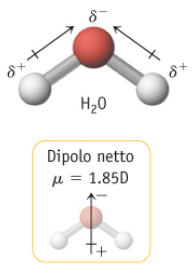
\includegraphics[width=5cm]{immagini/H_2O.png}
\end{figure}

\vspace{-0.4cm}Descrivendo l'acqua col formalismo di Lewis notavamo due coppie solitarie sull'ossigeno. Dovendo ragionare su un sistema con 4 coppie di elettroni usiamo l'idea del sistema tetraedrico nel quale però le due coppie solitarie stringono il legame, che avrà un angolo di 104.5°. Considerando solo gli atomi, questa molecola sarà piana ma angolata.

La differenza in elettronegatività tra idrogeno e ossigeno è cospicua, per cui entrambi i legami mostreranno un momento di dipolo. In questo caso però, a causa della geometria molecolare, la loro composizione dà luogo ad un momento di dipolo netto pari a 1.85D. Grazie ad esso l'acqua è la molecola che permette la vita.

\vspace{0.2cm}$\bullet$ ES7 BF$_3$

\begin{figure}[htp]
    \centering
    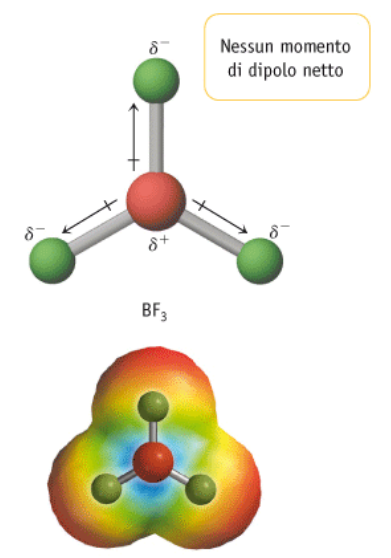
\includegraphics[width=6cm]{immagini/BF_3-dipolo.png}
\end{figure}

Nel descrivere tale molecola abbiamo detto che il boro presenta ibridizzazione sp$^2$, per cui essa sarà una molecola planare con angoli di 120°.

Il fluoro è parecchio più elettronegativo del boro, quindi ciascun legame mostrerà polarità, con la carica di legame addensata sul fluoro.

Essendo planare, la composizione dei tre momenti di dipolo, fra loro uguali in modulo, dà un momento di dipolo netto pari a zero, per cui il BF$_3$ non ha polarità. 

\vspace{0.2cm}$\bullet$ ES8 Cl$_2$CO
\begin{figure}[htp]
    \centering
    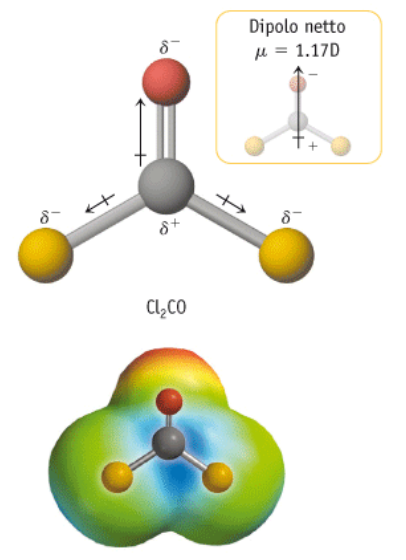
\includegraphics[width=6cm]{immagini/Cl_2CO.png}
\end{figure}

\vspace{-0.4cm}Nel fosgene un atomo di carbonio centrale è legato all'ossigeno tramite un doppio legame e a due atomi di cloro tramite due legami semplici. Sia il cloro che l'ossigeno sono parecchio più elettronegativi del carbonio, quindi ciascun legame mostrerà polarità con la freccia rivolta verso gli atomi esterni. Il momento di dipolo del legame carbonio-ossigeno è più forte, per cui la composizione darà un momento di dipolo netto pari a 1.17D.

\vspace{0.2cm}$\bullet$ ES9 NH$_3$

\begin{figure}[htp]
    \centering
    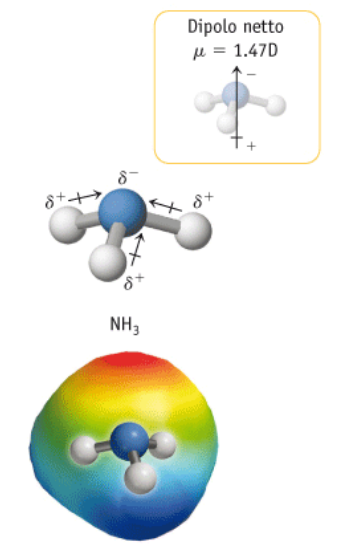
\includegraphics[width=6cm]{immagini/NH_3.png}
\end{figure}

\vspace{-0.4cm}Nell'ammoniaca è l'azoto centrale ad essere più elettronegativo, e lo è parecchio rispetto all'idrogeno. Ne segue che ogni legame mosterà polarità la cui freccia è rivolta verso questo. Inoltre col formalismo di Lewis abbiamo visto che su di esso è presente una coppia solitaria, la quale lo solleva dal piano dei tre atomi di idrogeno, per cui il momento di dipolo netto sarà diverso da zero.

Se non ci fosse stata la coppia solitaria, l'azoto si sarebbe disposto nel piano individuato dai 3 idrogeni come nel baso del \ce{BF_3} e quindi non si avrebbe avuto un momento di dipolo netto.

\vspace{0.2cm}$\bullet$ ES10 CH$_4$

\begin{figure}[htp]
    \centering
    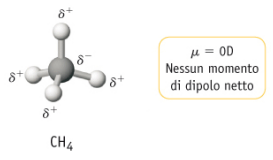
\includegraphics[width=5cm]{immagini/CH_4.png}
\end{figure}

\vspace{-0.4cm}Nel metano c'è una buona differenza in elettronegatività tra carobonio e idrogeno, ma a causa della sua geometria tetraedrica la risultante dei momenti di dipolo, uno per ciascun legame, sia pari a zero. Nei fatti il momento di dipolo osservato è zero.

\vspace{0.2cm}$\bullet$ ES11 CH$_3$Cl

\begin{figure}[htp]
    \centering
    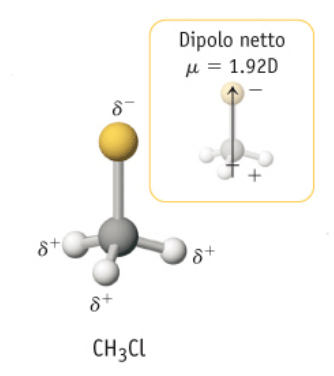
\includegraphics[width=5cm]{immagini/CH_3Cl.png}
\end{figure}

Se nel metano sostituiamo un idrogeno qualunque con un atomo di cloro, la molecola così ottenuta mostra un momento di dipolo netto. Il motivo è che il momento di dipolo del legame cloro-carbonio non è più equivalente agli altri tre, per cui nella loro composizione non si annullano a vicenda.

\vspace{0.2cm}$\bullet$ ES12 CH$_2$Cl$_2$

\begin{figure}[htp]
    \centering
    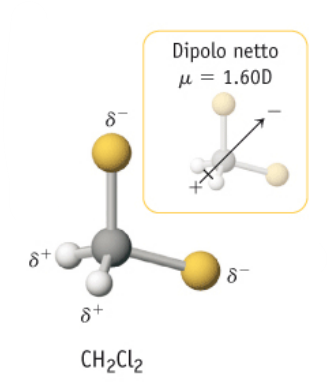
\includegraphics[width=5cm]{immagini/CH_2Cl_2.png}
\end{figure}

\vspace{-0.2cm}Se sostituiamo un secondo idrogeno con un altro atomo di cloro, la composizione dei momenti di dipolo ne darà uno netto ancora diverso da zero, sebbene minore rispetto al caso precedente.

\vspace{0.2cm}$\bullet$ ES13 CHCl$_3$

\begin{figure}[htp]
    \centering
    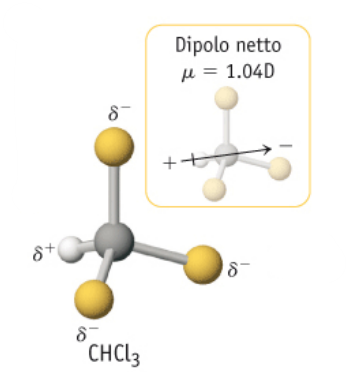
\includegraphics[width=5cm]{immagini/CHCl_3.png}
\end{figure}

Sostituendo anche un terzo idrogeno con un ulteriore atomo di cloro, la composizione dei momenti di dipolo sarà anche stavolta diversa da zero, ma ancora più piccola.

\vspace{0.2cm}$\bullet$ ES14 CCl$_4$

\begin{figure}[htp]
    \centering
    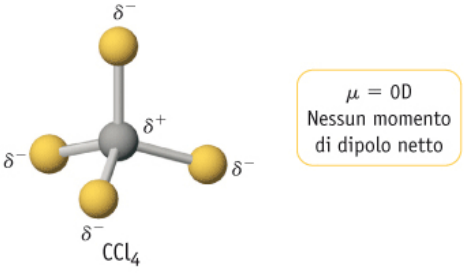
\includegraphics[width=5cm]{immagini/CCl_4.png}
\end{figure}

Nel momento in cui anche il quarto e ultimo idrogeno viene sostituito con un atomo di cloro otteniamo il tetracloruro di carbonio, il cui sistema sarà di nuovo simmetrico. Per esso la composizione dei momenti di dipolo sarà pari a zero, fatto confermato dalle evidenze sperimentali.

\vspace{0.2cm}$\bullet$ ES15 L'ordine di legame
\begin{figure}[htp]
    \centering
    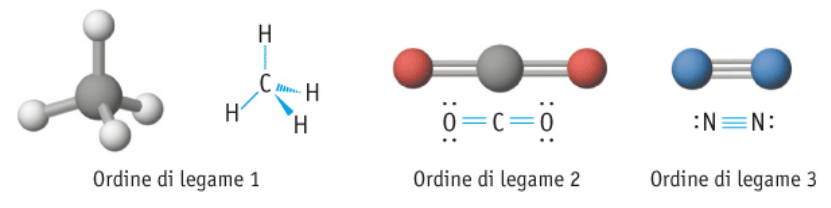
\includegraphics[width=14cm]{immagini/ordine-di-legame.png}
\end{figure}

Consideriamo queste molecole, in modo da dare nuovamente il cocnetto di ordine di legame. Diremo che un legame semplice ha ordine di legame 1, uno doppio ordine di legame 2 e uno triplo ordine di legame 3. Tuttavia nell'istante in cui ci fossero sistemi per i quali qualche doppio legame si possa ripartire su più legami semplici l'ordine non era più intero, ma frazionario
\subsection{Il legame ionico}
in esso la dislocazione delle cariche e totale, per cui immaginiamo che ci sia cessione dell'elettrone e in conseguenza a ciò si formino uno ione positivo e uno negativo.

\subsection{Considerazioni energetiche nella formazione di un legame ionico}
Immaginiamo di avere due atomi separati, ad esempio litio e fluoro.

Nella specie LiF sappiamo da altri studi che effettivamente si hanno ioni litio e fluoruro, ossia il litio ha ceduto il suo unico elettrone esterno al fluoro.

Se il litio cede un elettrone, vuol dire che è stata spesa dell'energia per strapparglielo, per esattezza si deve spendere una energia pari a quella di prima ionizzazione del litio, che ammonta a 520 kJ/mol.
Al contempo, poiché il fluoro sta acquistando un elettrone, dovrà emettere una certa quantità di energia pari alla sua affinità elettronica, che vale -328 kJ/mol. Questo significa che essa da sola non basta a ionizzare il litio, ossia se mettessimo vicini ma isolati due atomi, uno di fluoro e uno di litio, non si formerebbero questi ioni, in quanto il fluoro tenderebbe a catturare l'elettrone del litio, ma libererebbe un'energia non sufficiente a ionizzare il litio, poiché tale processo richiede più energia.

Ne segue che questi due atomi isolati non daranno luogo alla specie molecolare Li$^+$F$^-$.

Considerazioni analoghe valgono per qualsiasi altro composto ionico, come ad esempio l'NaCl: l'affinità elettrica del cloro non è sufficiente a strappare l'elettrone al sodio affinché diventi Na$^+$, in quanto il suo potenziale di prima ionizzazione è più altro dell'affinità elettronica del cloro, per cui la molecola NaCl non può esistere come singola entità.

Tuttavia sia il fluoruro di litio, che il cloruro di sodio, esistono.

Dobbiamo quindi trovare la fonte di questo legame, cioè capire perché esiste il solido ma non la molecola singola.

La prima domanda che quindi ci poniamo è: "Dove sta la forza che tiene legati insieme questi ioni, dato che il sistema solido esiste?"

Una prima risposta è che essa deve stare nella struttura adottata in fase solida. È lì che dobbiamo cercare la ragione, perché se la molecola non esiste e il solido si è chiaro che in quest'ultimo ci sarà un qualche contributo in energia che permette la formazione della specie chimica.

Per mostrare la validità di tale ipotesi utilizziamo un ciclo termodinamico, chiamato "\textbf{Ciclo di Born-Haber}", che permette di razionalizzare la ragione dell'esistenza dei solidi di tutti i sistemi ionici.

Il nostro obiettivo è capire perché possiamo prendere del litio solido Li$_{(s)}$, aggiungere del fluoro gassoso F$_{(g)}$ e ottenere il fluoruro di litio solido LiF$_{(s)}$ senza problemi.

Sappiamo però che il fluoruro di litio presenta una struttura solida nella quale ioni litio e ioni fluoruro occupano precise posizioni reticolari, quindi non è una struttura disordinata, anzi è estremamente ordinata.

L'energia che stiamo cercando è la variazione di entalpia che si ha nella formazione del solido ionico a seguito della reazione:
$$\ce{Li^{+}_{(g)} + F^{-}_{(g)} -> LiF_{(s)}} \quad \Delta\text{H=?}$$
In questa reazione una mole di litio gassoso reagisce con una mole di fluoro gassoso per dare luogo ad una mole di fluoruro di litio solido, in quanto non esiste in forma gassosa.

Purtroppo questa reazione è impossibile da realizzare perché in natura non abbiamo né ioni litio gassosi, in quanto in litio è presente solo come composto insieme a qualche altro elemento, né ioni fluoruro gassosi, in quanto esiste in forma molecolare F$_2$, per cui non possiamo partire da questi reagenti.

Quello che possiamo fare è partire dai composti del litio, fonderli, fare elettrolisi e ridurre il Li$^+$ a Li$^0$ tramite processi elettrochimici. Dopodiché facciamo reagire questo insieme al fluoro gassoso e otteniamo:
$$\ce{Li_{(s)} + \frac{1}{2}F_{2(g)} -> LiF_{(s)}}$$
Notiamo che questa reazione è diversa da quella di partenza, ma se stiamo attenti a lavorare a pressione costante, le energie scambiate diventano variazioni di entalpia $\Delta$H, che è una funzione di stato, per cui non dipenderà dal particolare percorso, ma solo da stato iniziale e finale. In altre parole possiamo fare avvenire questa reazione tramite il percorso diretto o tramite il percorso più complesso, contenuto all'interno del ciclo di Born-Haber, e la variazione di energia che si ha passando da reagenti a prodotti sarà la stessa.

Il processo che si usa è il seguente:
\begin{itemize}
    \item Si parte dal litio solido e si spende una certa energia $\Delta\text{H}_{atomiz}$ per portarlo in fase gassosa che chiamiamo energia di atomizzazione o evaporazione del litio, facilmente misurabile con un calorimetro.
    \item Si rompe la molecola biatomica del fluoro, passando così da F$_2$ a 2F. L'energia così spesa è quella di dissociazione del fluoro che è detta binding energy (BE). Poiché ci serve solo un atomo di fluoro e da ogni molecola ne otteniamo due, ci basta metà di questa energia.
    
    A questo punto avremo litio e fluoro entrambi allo stato gassoso.
    \item Si fornisce l'energia di prima ionizzazione $IP_1$ del litio per ottenere il suo catione:
    
    \ce{Li_{(g)} -> Li^{+}_{(g)} + 1e}
    \item L'elettrone ottenuto dalla ionizzazione del litio viene acquistato dal fluoro, il quale diventa F$^-$ e cede un'energia pari alla sua affinità elettronica $EA$.
    \item Arriviamo così ad avere ioni $Li^+$ e $F^-$ gassosi, che sono i reagenti della reazione considerata inizialmente, la quale ci interessa poiché in essa vi è tutta la stabilità del sistema solido.
    
    Essi insieme daranno luogo al fluoruro di litio solido e quindi pur non avendo fatto il percorso diretto siamo arrivati allo stesso prodotto:
\end{itemize}

\begin{figure}[htp]
    \centering
    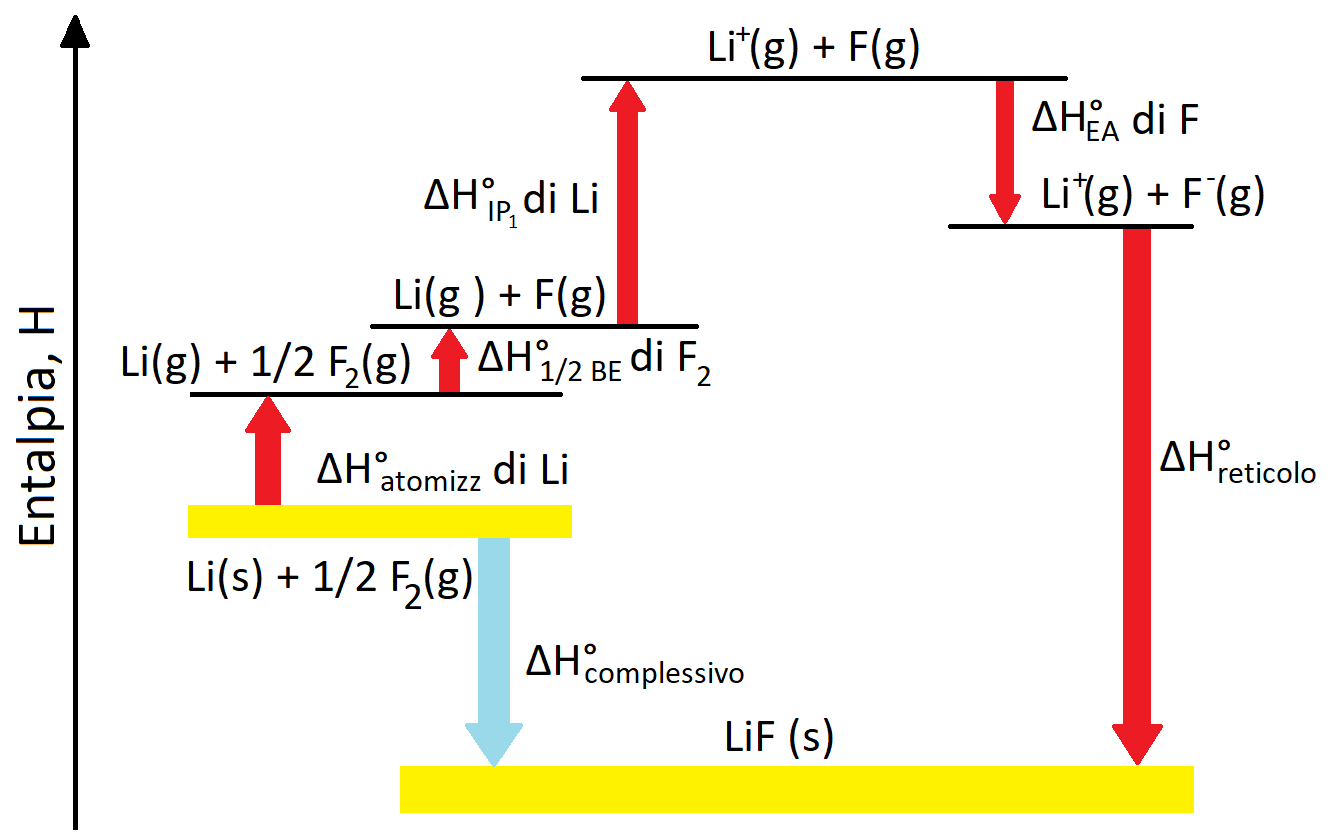
\includegraphics[width=10cm]{immagini/Ciclo-Born-Haber.png}
\end{figure}

Poiché stato iniziale e stato finale sono gli stessi, la somma di tutti questi calori deve essere uguale al calore scambiato nel percorso diretto.

Il calore di formazione emesso nel processo diretto lo sappiamo calcolare, mentre nel processo complesso non sappiamo misurare solo il calore emesso per passare dagli ioni gassosi al reticolo solido, la quale però può essere calcolata facendo la differenza tra valori sperimentali:
$$\Delta\rm{H}_{reticolo}=\Delta\rm{H}_{complessivo} - \Delta\rm{H}_{atomiz} - \Delta\rm{H}_{BE} - \Delta\rm{H}_{IP_1} + \Delta\rm{H}_{EA}$$
Si trova che, alla temperatura di 25° C e alla pressione di 1 bar, il $\Delta\rm{H}$ complessivo è pari a -617 kJ/mol. È negativo perché quando mettiamo insieme litio e fluoro spontaneamente si forma il fluoruro di litio, emettendo tale calore.

Facendo la differenza tra tale calore e gli altri calori misurabili si trova che l'energia di reticolo vale -1050 kJ/mol, che viene emessa con la formazione del reticolo.

Quindi il legame chimico nei sistemi ionici sta tutto nella formazione del reticolo, cioè la stabilità del solido e la inesistenza della singola molecola sta nel fatto che in questa l'energia emessa dal fluoro quando acquista un elettrone non basta a ionizzare il litio, che è quello che dovrebbe cedere l'elettrone, per cui la molecola non potrà formarsi, mentre quando si forma il solido questi ioni liberano una grande quantità di energia, cosa che permette al solido di formarsi. Quindi è proprio all'interno del reticolo che si trova la stabilità di questo sistema: quando questi ioni vanno ad occupare precise posizioni reticolari si forma questo reticolo estremamente stabile con l'emissione di una quantità molto grande di energia.

Questo discorso vale per tutti i solidi ionici: non esistendo le loro molecole ma il loro solido si, vuol dire che la stabilità è conferita dall'arrangiamento in fase solida.

\textbf{Legge di Hess}: il calore scambiato a pressione costante in una reazione chimica che possa essere scomposta in più reazioni parziali è indipendente dagli stati intermedi attraverso i quali si evolve il sistema e dipende solo dagli stati iniziale e finale. La variazione di calore è pari alla somma algebrica delle variazioni di calore dei singoli stadi.

A causa di tale legge, se abbiamo calori scambiati a pressione costante il sistema può essere rappresentato attraverso una serie di stati intermedi, ottenendo così un ciclo termodinamico e quindi le energie coinvolte dipendono solo dallo stato iniziale e da quello finale.

\vspace{0.2cm}N.B.: Se chiede di parlare del legame ionico attraverso un modello termodinamico descrivi il ciclo, ma se chiede perché abbiamo la necessità di usare il ciclo, il motivo è perché siamo interessati al $\Delta\rm{H}_{reticolo}$, che è l'energia del reticolo cristallino, perché in tale reazione da un lato abbiamo gli ioni gassosi e dall'altro li abbiamo nel solido, nel reticolo cristallino, per cui vogliamo conoscere l'energia che viene emessa quando questo si forma, ossia partiamo da un'energia molto alta di questi ioni $Li^+$ e $F^-$ gassosi e quando questi si uniscono per formare il solido emettono una quantità enorme di energia, e il sistema si stabilizza tantissimo. Questa energia emessa si chiama "energia reticolare" perché è l'energia del reticolo. Quindi in questo secondo caso la prima cosa da dire è:"l'energia reticolare è l'energia associata al processo nel quale sono reagenti, in questo caso particolare, ione litio gassoso più ione fluoruro gassoso, e il prodotto è il fluoruro di litio, ma noi non siamo in grado di effettuare questa reazioni, perché questi reagenti non li abbiamo. Ecco perché usiamo il ciclo di Born-Haber, il quale mi permette di aggirare questo problema". Dopodiché si  inizia a parlare del ciclo, quindi diamo la motivazione (voler conoscere l'energia del reticolo, che è quella che tiene insieme gli ioni nel reticolo).

\subsection{Differenze tra composti molecolari e composti ionici}
Per i composti molecolari esistono le singole molecole, per quelli ionici no: essi esistono solo in forma di reticolo cristallino, dove gli ioni occupano posizioni ben precise, alternandosi, in tutte e 3 le direzioni.

La conseguenza di ciò è che se mettiamo in acqua ad esempio il glucosio \ce{C_6H_{12}O_6}, che è un composto molecolare, esso resta tale, mentre se mettiamo ad esempio il cloruro di sodio NaCl esso si dissocia in ioni Na$^+$ e Cl$^-$. Ciò che avviene è che l'acqua aggredisce il cristallo e stacca singoli ioni, i quali vengono portati in soluzione con delle molecole di acqua che li circondano. In particolare gli ioni positivi saranno circondati dagli atomi di ossigeno dell'acqua, in quanto essi reagiranno con la parziale carica negativa presente su questo, mentre gli ioni negativi saranno, mentre gli ioni negativi saranno circondati dagli idrogeni dell'acqua poiché interagiranno con la parziale carica positiva presente su questi:
\begin{figure}[htp]
    \centering
    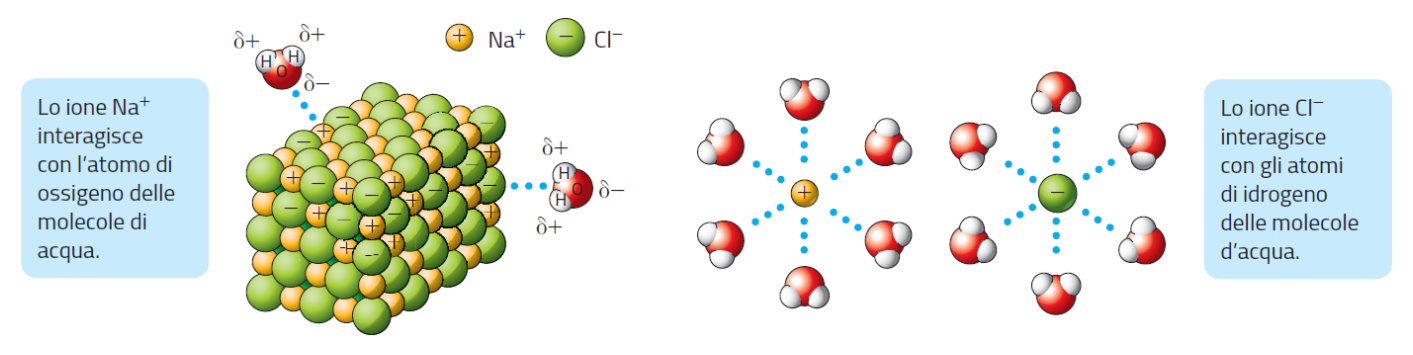
\includegraphics[width=15cm]{immagini/interazione-acqua-ioni.png}
\end{figure}
Dunque in soluzione si avranno ioni.

L'evidenza sperimentale di tale fatto si ottiene confrontando tre circuiti elettrici con una lampadina, dove in uno inseriamo in serie dell'NaCl solido, in un altro dell'NaCl fuso e in un terzo una soluzione di NaCl sciolto in acqua. Il primo non permette la conduzione (la lampada non si accende), il secondo permette una leggera conduzione (la lampada si accende ma la luce è fioca), il terzo permette una grande conduzione (la lampada si accende con luminosità maggiore).

\begin{figure}[htp]
    \centering
    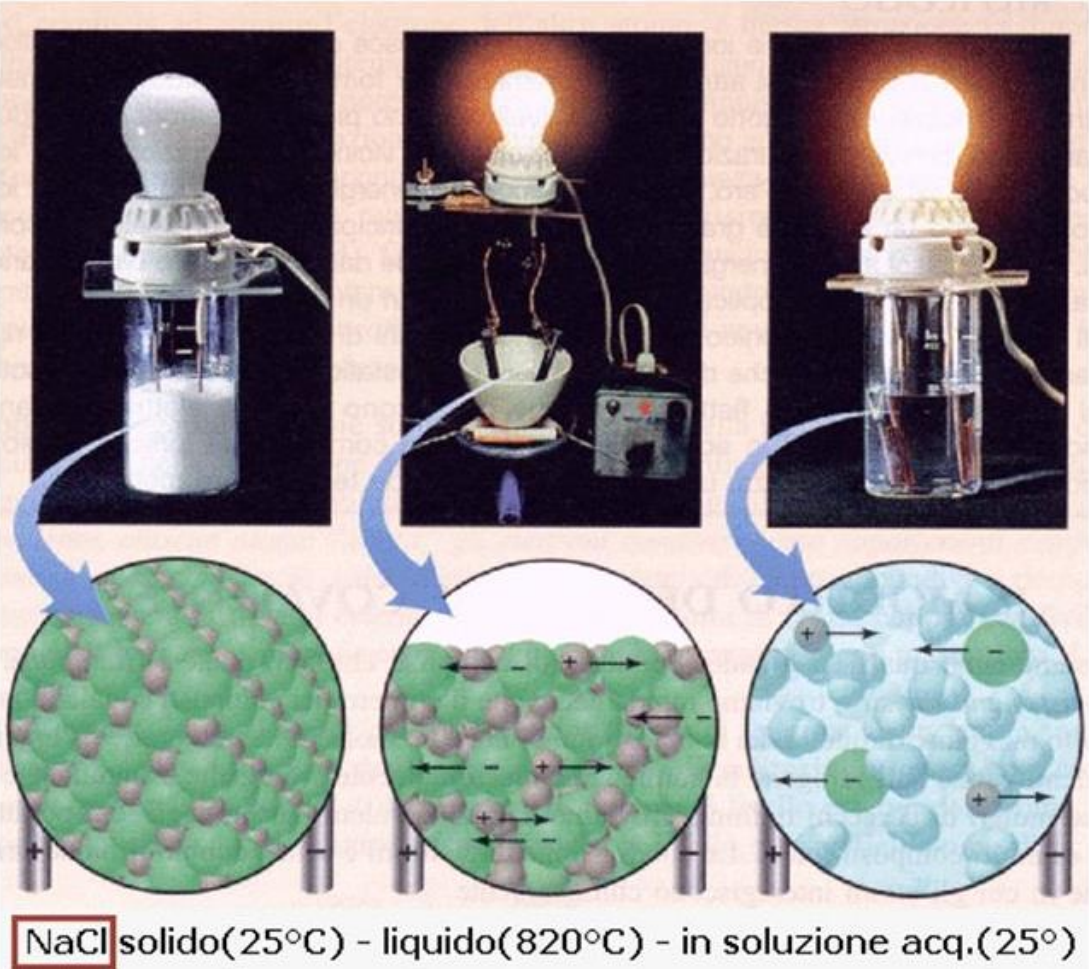
\includegraphics[width=10cm]{immagini/lampadina.png}
\end{figure}

Tale esperimento mostra l'esistenza degli ioni, che sono i portatori di carica che permettono la conduzione.

Se invece avessimo collegato a lampadina ad una soluzione acquosa contenente zucchero, la lampadina non si accenderebbe. Il motivo è che lo zucchero è un composto molecolare, per cui non si scioglie in acqua e non dà origine a ioni.
\subsection{Proprietà fisiche dei composti ionici}
Tipicamente i composti ionici sono duri, rigidi e fragili, cioè è facile romperli.

Se solidi, non conducono elettricità, per cui costituiscono dei buoni isolanti. Se invece li portiamo a fusione (che per tali composti significa portarli ad una temperatura di 800-1000°C) iniziano a condurre. Se invece li sciogliamo in acqua la mobilità degli ioni diventa elevata e la conducibilità è ancora maggiore. Tale fatto è la dimostrazione dell'esistenza degli ioni come portatori di carica.

In genere hanno temperature di fusione elevate, perché dobbiamo abbattere l'energia reticolare, che è molto elevata, per poter liberare gli ioni dal reticolo.

All'interno dei reticoli gli ioni sono disposti alternatamente nelle varie direzioni
\begin{figure}[htp]
    \centering
    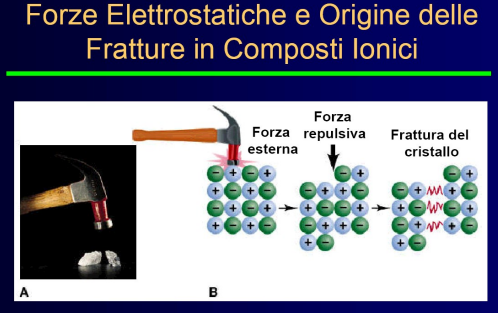
\includegraphics[width=10cm]{immagini/struttura-composti-ionici.png}
\end{figure}
Immaginiamo un sistema bidimensionale. Se cerchiamo di rompere il cristallo, lo si deve spezzare e far scivolare il sistema in un piano. Se riusciamo a fare ciò, riusciamo a rompere il cristallo.
\subsection{Il modello del legame covalente}
Consideriamo due atomi di idrogeno, che immaginiamo inizialmente posti a distanza infinita, i quali via via si avvicinano. Nella situazione iniziale possiamo dire che non esiste alcuna interazione fra i due atomi, ma nell'istante in cui la distanza, pur grandissima che sia ma comunque finita, i due atomi iniziano ad interagire.

Il grafico dell'energia potenziale ha il seguente andamento:
\begin{figure}[htp]
    \centering
    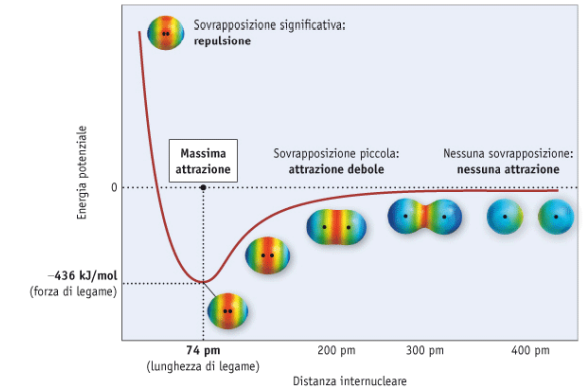
\includegraphics[width=10cm]{immagini/energia-potenziale.png}
\end{figure}

Essa sarà l'energia di due atomi di idrogeno che si avvicinano.

Inizialmente abbiamo valori di energia prossimi a zero, ossia quando la distanza è infinita questo sistema ha energia potenziale nulla. Nell'istante in cui la distanza diventa misurabile i due atomi iniziano ad interagire. Ciò significa che quando i due atomi si avvicinano si può già parlare di energia negativa e quindi i due atomi si stanno realmente legando, ossia possiamo immaginare che si inizi ad instaurare un legame chimico.

I due atomi si avvicineranno fino ad una certa distanza in cui si ha il minimo di energia per il sistema. Per due atomi di idrogeno legati si ottiene quando la distanza di equilibrio (perché i due atomi vibrano, non sono rigidamente fermi) è pari 0.74 Å.

Se tentassimo di avvicinarli ulteriormente, l'energia inizierebbe a crescere velocemente superando persino lo zero, perché inizia ad essere incisiva la repulsione tra i nuclei e tra gli elettroni. Se invece li allontanassimo l'energia tenderebbe al valore U=0, che prende il nome di "asintoto di dissociazione", e i due atomi non sarebbbero più legati.

Nel punto di minimo di energia per due atomi di idrogeno si trova un valore di -436 kJ/mol, che è il valore di energia che dovremmo spendere per rompere il legame della molecola H$_2$.

\vspace{0.2cm}
Seguendo questa curva sembrerebbe che siano possibili tutte le energie, ma non è così. Infatti abbiamo detto che l'energia è quantizzata, e tale è anche l'energia di vibrazione di due atomi di idrogeno all'interno di una molecola di H$_2$, per cui solo alcuni dei valori rappresentati sono permessi. Questo modo di rappresentare l'energia è più adatto per un sistema macroscopicom i cui valori di energia non siano quantizzati. Tuttavia si usa comunque questa rappresentazione per sistemi quantizzati, dato che i valori possibili di energia stanno su questa curva.
\begin{figure}[htp]
    \centering
    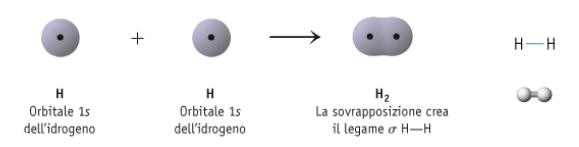
\includegraphics[width=10cm]{immagini/legame-H_2.png}
\end{figure}

Quello che quindi stiamo immaginando è di avere due atomi di idrogeno con due orbitali 1s, ciascuno con un proprio elettroni. Questi due orbitali interagiscono dra di loro per dar luogo alla formazione di un legame chimico, con l'ottenimento della molecola H$_2$. Se abbiamo due orbitali di tipo $s$, cioè a simmetria sferica, si ottiene un legame di tipo $\sigma$, che è quello che rappresentiamo come una lineetta tra i due atomi di idrogeno. 

\vspace{0.2cm}Consideriamo adesso l'acido fluoridrico HF. Il fluoro è il primo degli alogeni. Ha orbitali 2s e 2p come orbitali di valenza. L'orbitale 2s è parecchio interno come energia, quindi non adatto per interagire con l'orbitale 1s dell'atomo di idrogeno. Abbiamo poi i tre orbitali $p$: uno di questi avrà i suoi lobi orientati lungo quello che etichettiamo "asse di legame". L'orbitale p del fluoro orientato lungo tale asse, interagirà con l'orbitale 1s dell'idrogeno e formerà un legame $\sigma$, perché si ha sovrapposizione lungo l'asse di legame, sebbene gli orbitali interagenti siano uno di tipo $s$ e uno di tipo $p$
\begin{figure}[htp]
    \centering
    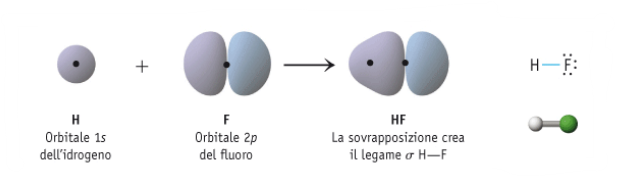
\includegraphics[width=10cm]{immagini/legame_H-F.png}
\end{figure}

Va da notare che i due lobi dell'orbitale p hanno colori diversi, e ad interagire con l'orbitale s dell'idrogeno è quello che ha lo stesso colore di ques'ultimo. Il motivo è che i lobi degli orbitali p hanno segno opposto, pertanto affinché i due orbitali interagiscano si deve scegliere il lobo avente lo stesso segno.

\vspace{0.2cm} Prendiamo adesso in esame la molecola F$_2$. Essendo due atomi identici avranno gli stessi orbitali, e in particolare quelli più esterni nel fluoro sono i $p$. Per ciascun atomo di fluoro, uno dei tre giacerà lungo l'asse di legame:
\begin{figure}[htp]
    \centering
    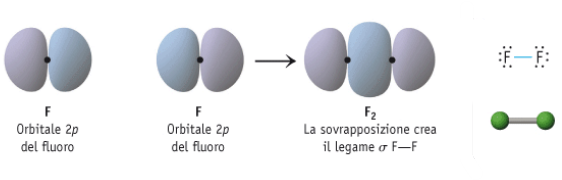
\includegraphics[width=10cm]{immagini/legame-F_2.png}
\end{figure}

Se li orientiamo in modo tale che i lobi che si affacciano l'uno sull'altro abbiano lo stesso segno ancora una volta otterremo un orbitale $\sigma$, in quanto ci sarà addensamento lungo la congiungente i due nuclei cioè lungo l'asse di legame, nonostante esso si stia formando tramite due orbitali $p$.

\vspace{0.2cm} Da questi esempi deduciamo che il legame $\sigma$ non necessariamente debba venir fuori da due orbitali di tipo s, ma può venir fuori anche un orbitale $s$ e uno $p$ o da due orbitali $p$. La cosa fondamentale è che gli orbitali che interagiscono siano orientati lungo la stessa direzione.
\subsection{Gli orbitali molecolari}
La teoria degli orbitali molecolari considera la molecola come un insieme di nuclei e di elettroni e,
valutando le loro reciproche interazioni, determina le funzioni d’onda che descrivono gli elettroni nella
molecola in modo analogo a quello usato per individuare le funzioni d’onda che descrivono gli elettroni
negli atomi isolati.

\vspace{0.2cm}Consideriamo la molecola più semplice che esista: la molecola H$_2^+$. Il motivo per cui consideriamo lo ione piuttosto che la molecola H$_2$ è che questa è composta da due atomi di idrogeno, ognuno dei quali porta un elettrone, per cui nel complesso avremo due protoni e due elettroni, mentre nello ione abbiamo un solo elettrone. Tale fatto ci permette di studiarla tramite l'equazione di Schrödinger, per cui siamo in grado di ottenere le soluzioni esatte delle sue energie.

In termini semplici, l'atomo di idrogeno consiste di un protone e un elettrone. Nell'istante in cui abbiamo due protoni, quali energie bisogna considerare?

Una prima energia sarà data dall'attrazione tra l'elettrone con il nucleo dell'atomo di idrogeno A. Tale contributo è negativo e abbassa l'energia del sistema:

\begin{figure}[htp]
    \centering
    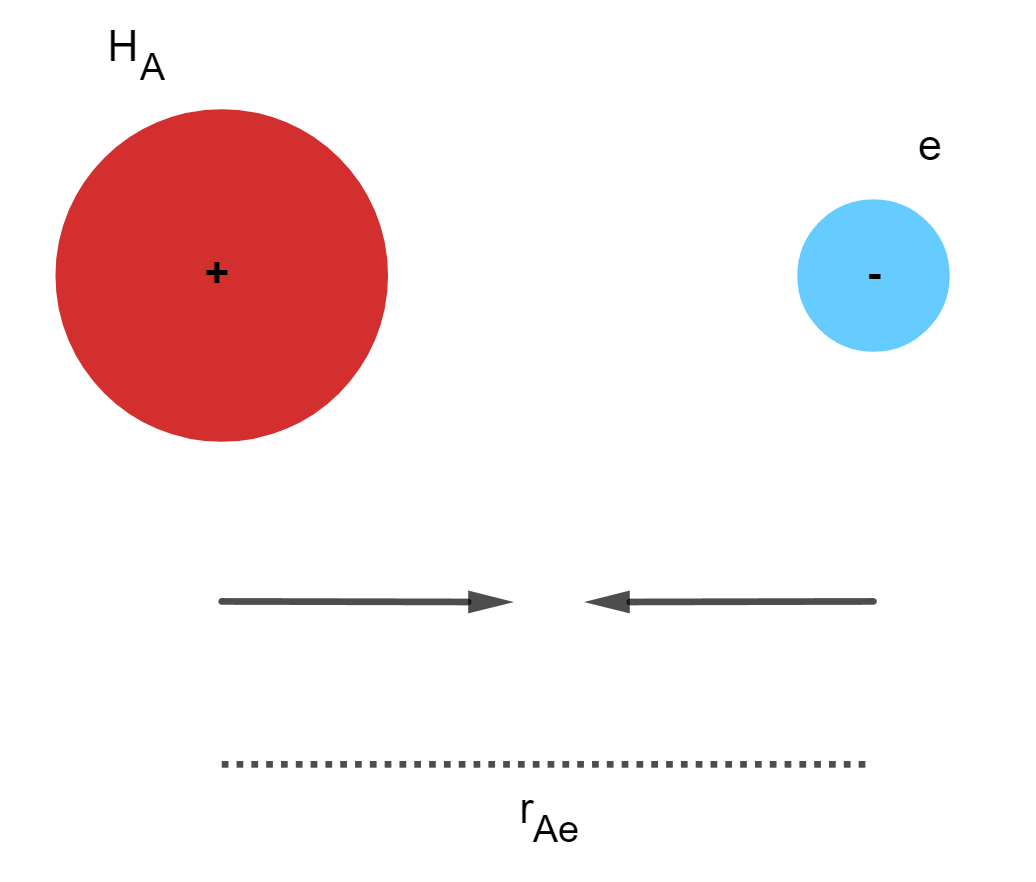
\includegraphics[width=5cm]{immagini/attrazione protone-elettrone.png}
\end{figure}

Tale energia vale $E=\displaystyle-\frac{q^2}{r_{Ae}}$.

Un secondo contributo analogo si avrà dall'attrazione tra elettrone e atomo di idrogeno B: $E=\displaystyle-\frac{q^2}{r_{Be}}$

\vspace{0.2cm}Un terzo e ultimo contributo sarà dato dalla repulsione tra i due nuclei. Esso sarà positiva, quindi alzerà l'energia:
\begin{figure}[htp]
    \centering
    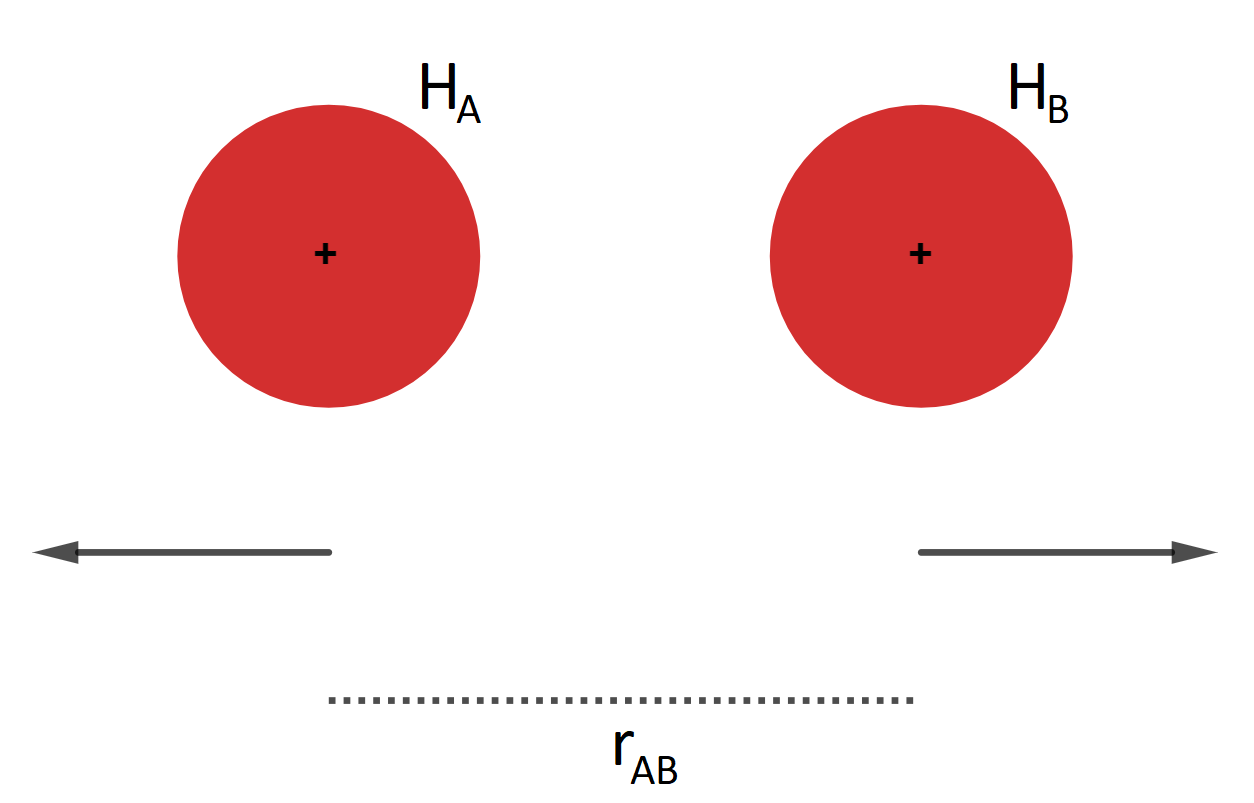
\includegraphics[width=6cm]{immagini/repulsione protone-protone.png}
\end{figure}

Tale energia vale $E=\displaystyle-\frac{q^2}{r_{AB}}$.

\vspace{0.2cm}L'elettrone quindi interagisce con entrambi i nuclei:
\begin{figure}[htp]
    \centering
    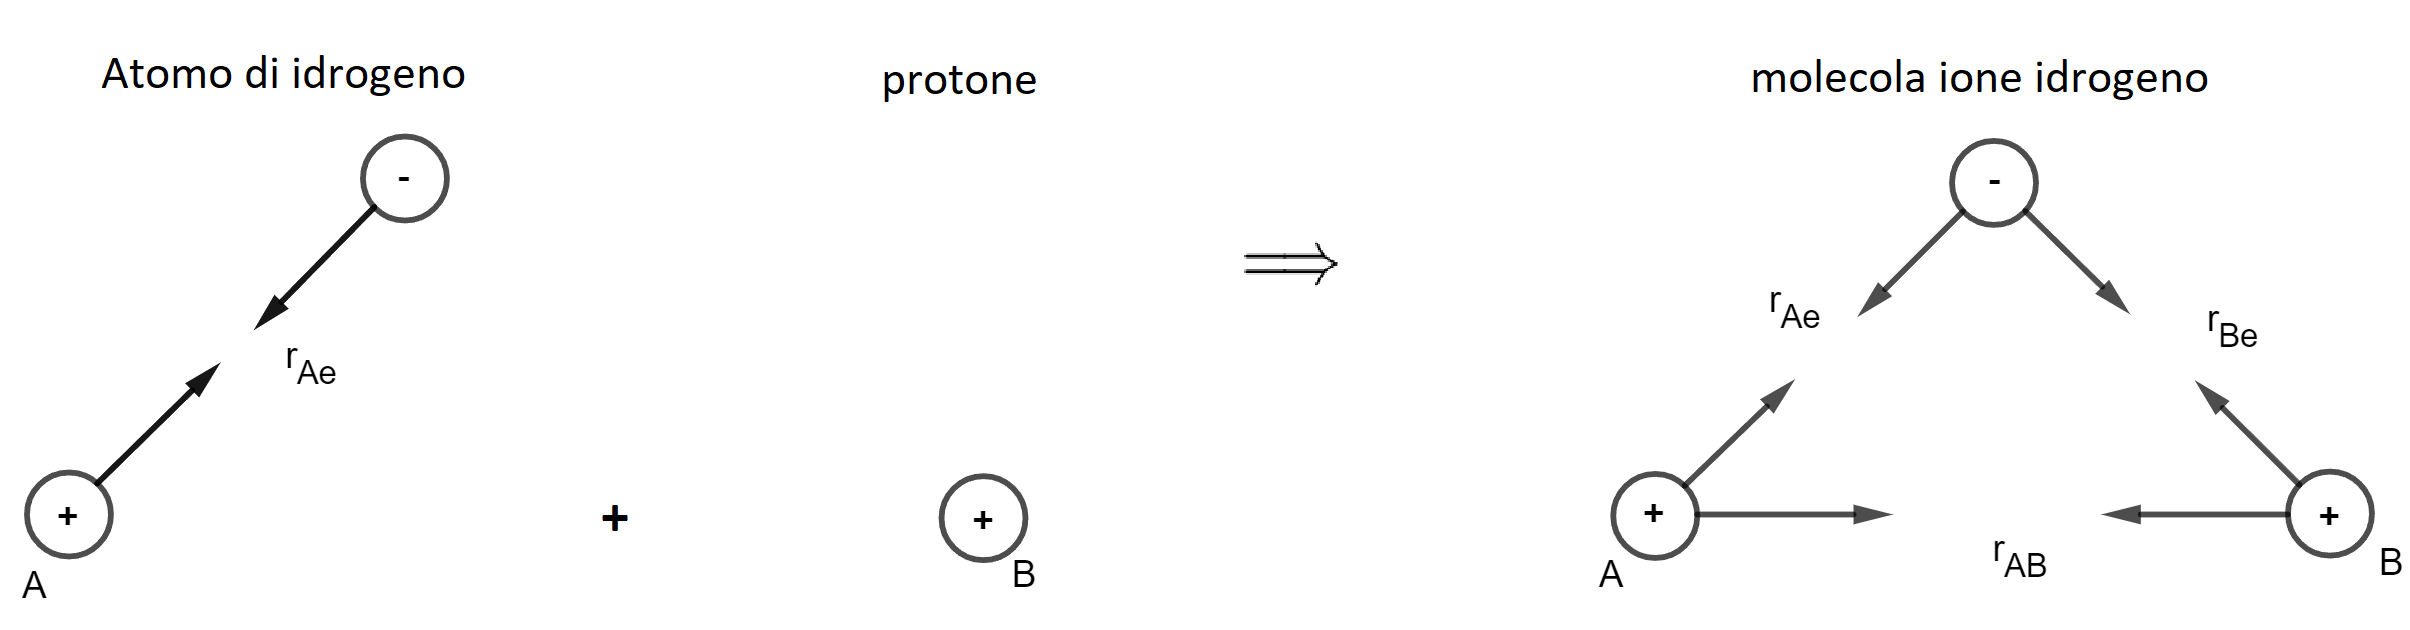
\includegraphics[width=14cm]{immagini/interazione_elettrone_con_protoni.png}
\end{figure}

Avremo tre distanze: quella tra il nucleo A e l'elettrone $r_Ae$, quella tra il nucleo B e l'elettrone $r_Be$ e quella tra i due nuclei $r_AB$.

Va da ricordare che la meccanica quantistica studia stati stazionari, cioè indipendenti dal tempo, il che significa che stiamo immaginando la molecola come se fosse rigida, cioè nel momento in cui andiamo a fare questi calcoli immaginiamo che non esistano vibrazioni ecc.

I termini energetici che avremo sono:
$$\ce{H_A^+-H_B^+ \quad + \quad H_A^+-e^- \quad + \quad H_B^+-e^-}$$
$$\text{repulsione \qquad attrazione \qquad attrazione}$$
$$\frac{q^2}{r_{AB}} \qquad - \qquad \frac{q^2}{r_{Ae}} \qquad - \qquad \frac{q^2}{r_{Be}}$$

Se immmaginiamo di avere particelle in posizioni fissate, possiamo andare a vedere qual è la composizione delle forze.

\begin{figure}[htp]
    \centering
    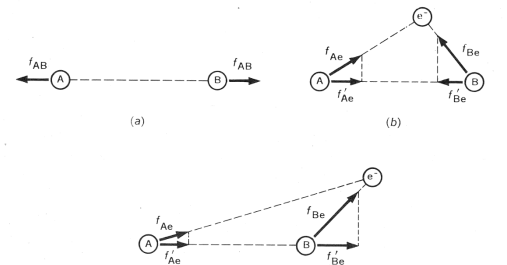
\includegraphics[width=10cm]{immagini/posizone_elettrone.png}
\end{figure}

Si nota che se questo elettrone, anziché essere fra i due nuclei fosse in una regione diversa (ad esempio a destra del nucleo B) sentirebbe l'attrazione di un nucleo, ma non è detto che senta quella dell'altro.

Quindi formalmente se l'elettrone viene immaginato come una particella, è chiaro che la sua posizione nello spazio è importante.

\vspace{0.2cm}Secondo la teoria degli orbitali molecolari, quando si formano molecole il numero di orbitali che ogni atomo possiede contribuirà agli orbitali molecolari che troveremo sulla molecola. Questo significa che se un atomo ha n orbitali di valenza, tutti questi contribuiranno a formare un ugual numero di orbitali molecolari.

In questo esempio abbiamo un orbitale $1s$ su ciascun atomo di idrogeno, per cui otterremo due orbitali molecolari: avremo una combinazione detta "\textit{in fase}" delle funzioni d'onda $1s_A + 1s_B$, e una combinazione detta  \textit{fuori fase} delle funzioni d'onda $1s_A - 1s_B$. La prima è detta \textit{combinazione di legame}, la seconda di \textit{antilegame}. In termini spaziali significa che per una data molecola lo spazio si divide in due regioni che daranno luogo, se è lì presente l'elettrone, alla combinazione legante e a quella antilegante:

\begin{figure}[htp]
    \centering
    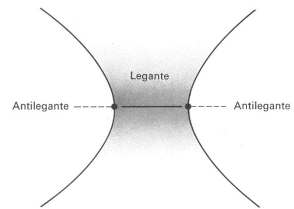
\includegraphics[width=6cm]{immagini/spazio_legante_antilegante.png}
\end{figure}

L'orbitale di antilegame si chiama così perché riempirlo non dà forza, anzi tende a distruggere il legame, a differenza di quello di legame che se riempito rafforza il legame.

Ne segue che di volta in volta dovremo fare i conti, in modo da capire quanti sono gli orbitali interagenti e quanti elettroni abbiamo a disposizione, in quanto le proprietà del legame dipenderanno da quanti orbitali di legame e quanti di antilegame si riempiranno.

\vspace{0.2cm}Sappiamo che sovrapporre due orbitali atomici di tipo $s$ significa ottenere orbitali molecolari di tipo $\sigma$. Supponiamo di avere due atomi di idrogeno distanti. Man mano che li avviciniamo, anche i loro orbitali atomici si avvicineranno, fino a sovrapporsi. Se ricordiamo l'andamento dell'energia potenziale, essa ha un minimo ad una distanza ben precisa sopra e sotto la quale l'energia è maggiore:

\begin{figure}[htp]
    \centering
    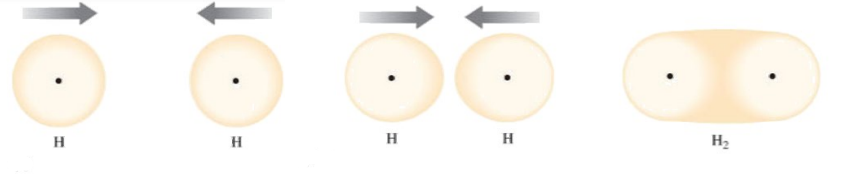
\includegraphics[width=12cm]{immagini/avvicinamento_orbitali.png}
\end{figure}

Supponiamo di essere alla distanza esatta che produce un minimo di energia. Essendoci un addensamento lungo la congiungente i nuclei ovvero lungo l'asse di legame, si ha un'interazione di tipo $\sigma$.

\vspace{0.2cm}Anche un orbitale $s$ con un orbitale $p$, e persino anche due orbitali $p$ orientati entrambi lungo l'asse di legame, danno luogo a un'interazione $\sigma$ che produce due orbitali: uno di legame  $\sigma$ e uno di antilegame  $\sigma^*$.

\begin{figure}[!tbp]
    \centering
    {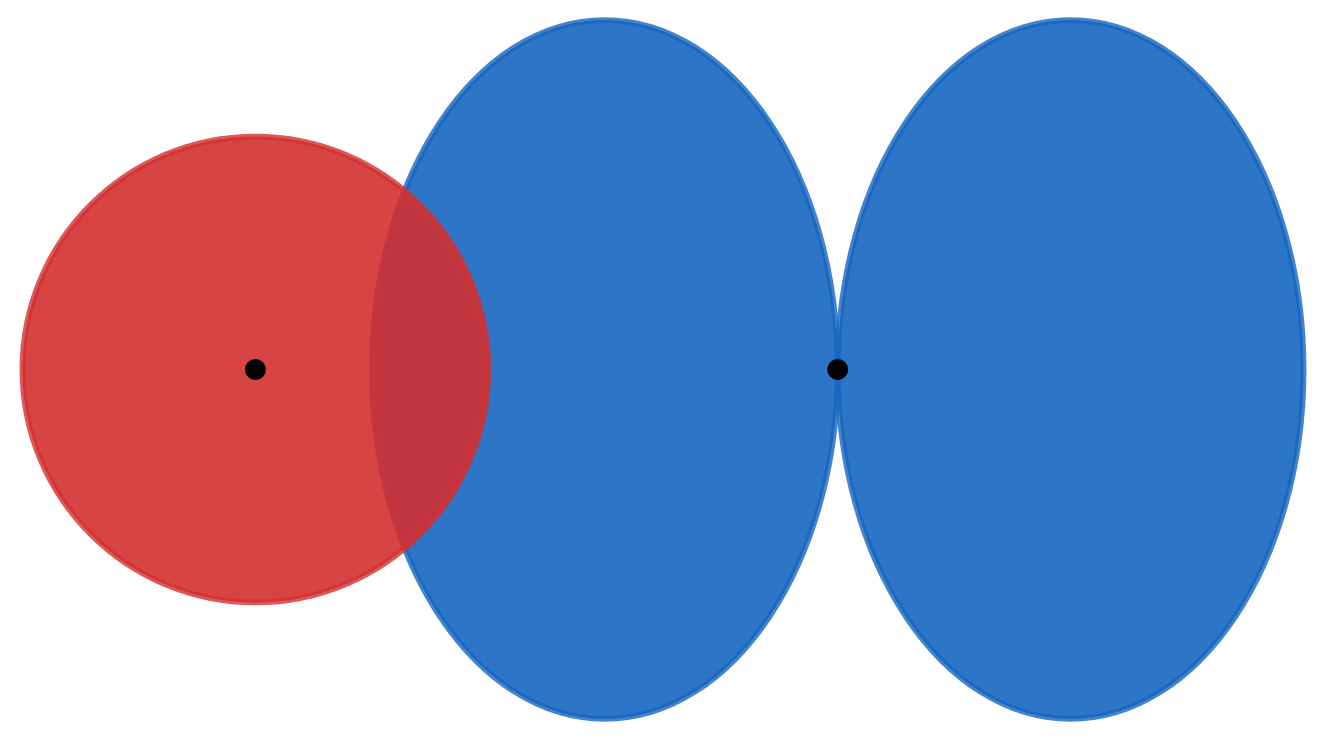
\includegraphics[width=4cm]{immagini/legame_sigma_s_p.png}\label{fig:f1}}
    \hfill
    {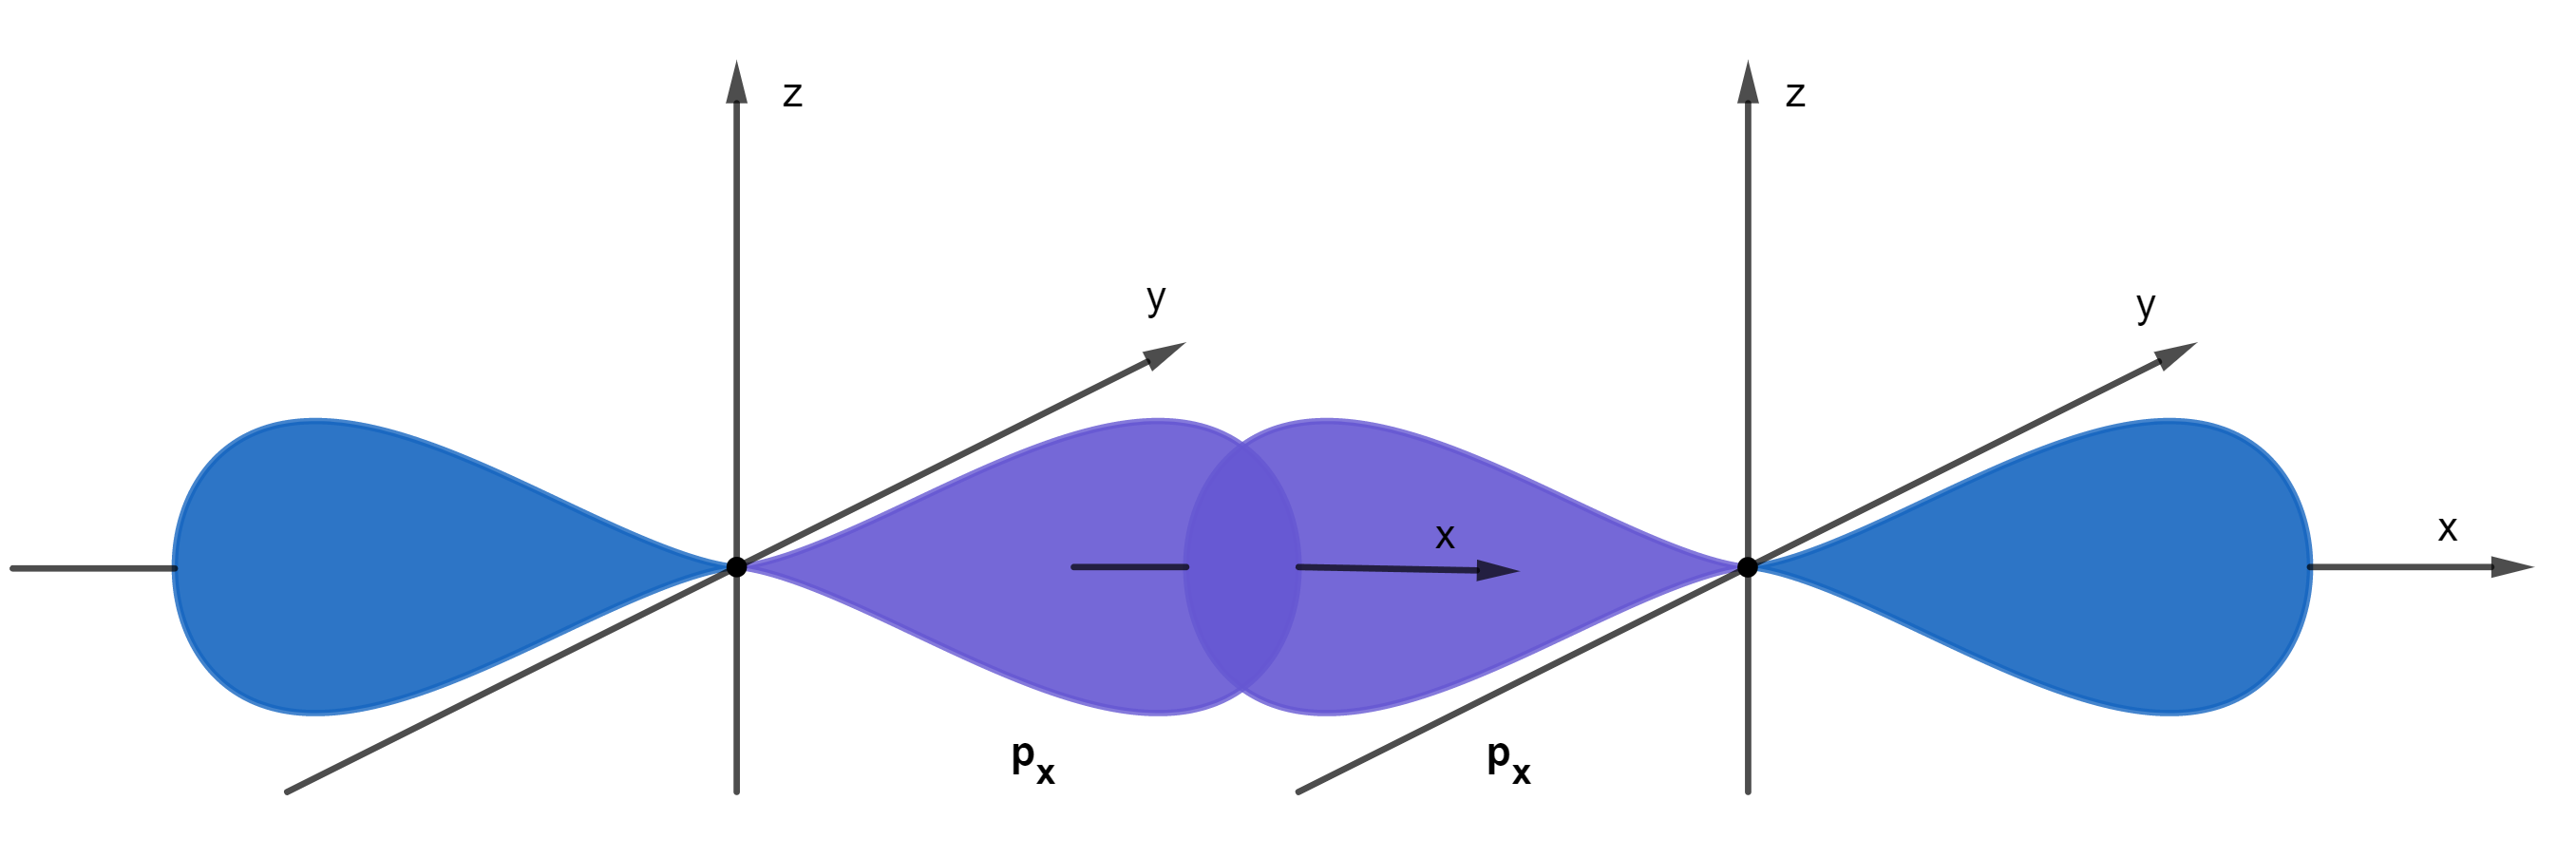
\includegraphics[width=10cm]{immagini/legame_sigma_p_p.png}\label{fig:f2}}
  \end{figure}

(Nel grafico è riportata solo la combinazione di legame).
L'orbitale molecolare di legame sarà quello nel quale i lobi degli orbitali atomici interagenti (cioè le funzioni d'onda) hanno lo stesso segno, mentre in quello di antilegame hanno segno opposto.

Nel caso di interazione $\sigma$ tra due orbitali $p$, se abbiamo stabilito (come nel caso del grafico) che questi siano orientati lungo l'asse x, gli orbitali $p_y$ e $p_z$ saranno perpendicolari a tale asse e daranno lugo a sovrapposizioni $\pi$:

\begin{figure}[!tbp]
    \centering
    {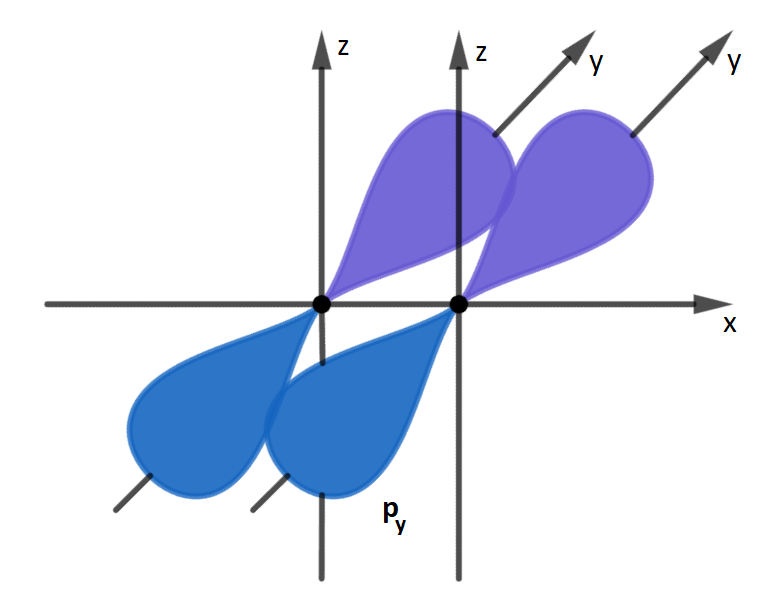
\includegraphics[width=7cm]{immagini/orbitali_py.png}\label{fig:f3}}
    \hfill
    {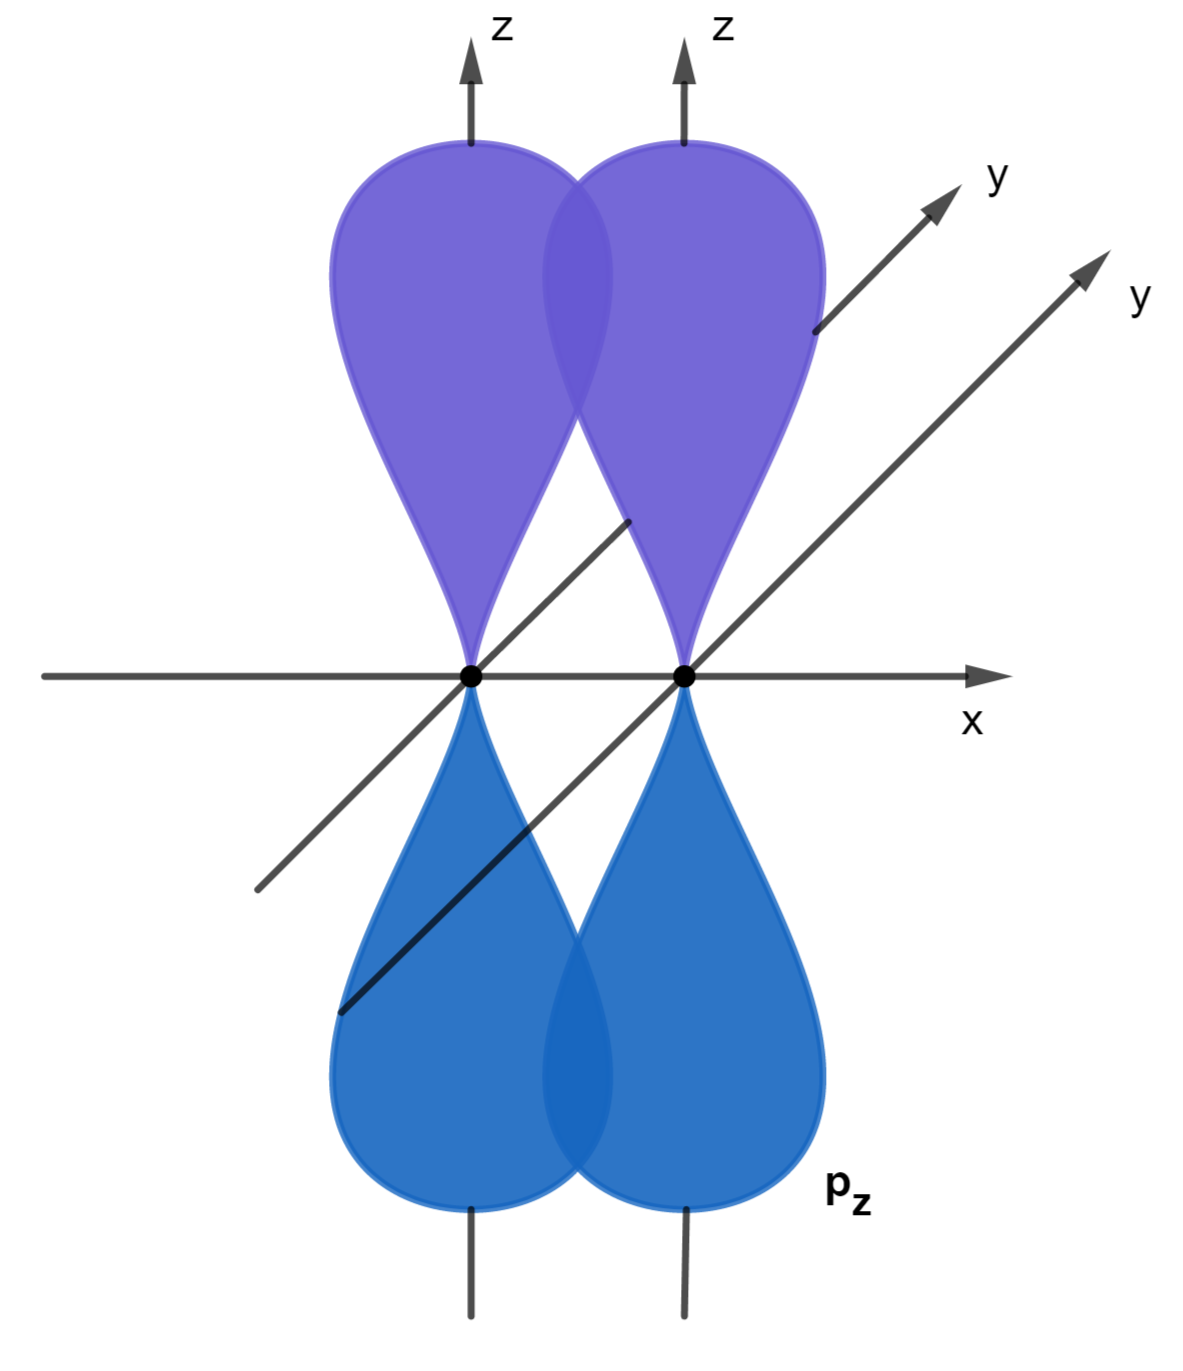
\includegraphics[width=5cm]{immagini/orbitali_pz.png}\label{fig:f4}}
\end{figure}

Quindi per una coppia di orbitali $p$ avremo una sovrapposizione diretta lungo la congiungente i due nuclei, mentre per le altre due coppie la sovrapposizione avverrà sopra e sotto.
\subsubsection{Forze attrattive e repulsive nel legame covalente}
\begin{figure}[!tbp]
    \centering
    {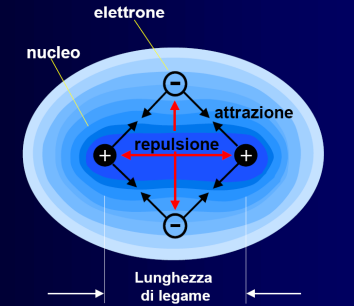
\includegraphics[width=5cm]{immagini/forze_legame_covalente.png}\label{fig:f5}}
    \hfill
    {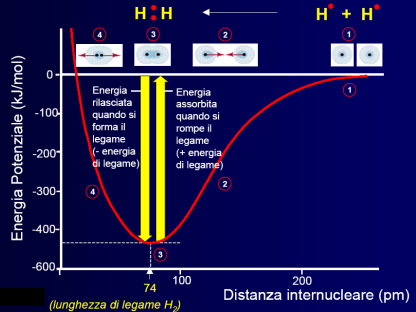
\includegraphics[width=10cm]{immagini/legame_covalente_H_2.png}\label{fig:f6}}
\end{figure}

Questo è il modello che dobbiamo considerare quando studiamo composti nei quali il legame è covalente.

In questo caso non stiamo parlando di cessione di elettroni come invece se ne parla nel legame ionico.

Se abbiamo due nuclei di idrogeno e due elettroni, questi ultimi daranno luogo a forze attrattive in certe posizione rispetto ad altre.

Ruguardiamo la formazione della molecolaH$_2$: due atomi di idrogeno inizialmente molto distanti hanno energia potenziale praticamente nulla, ossia non interagiscono. Iniziamo ad avvicinare i due atomi e l'energia potenziale si abbassa. Appena le avviciniamo fino a 0.74 Å raggiungiamo il minimo. Si sono così formati i due orbitali molecolari, uno di legame e uno di antilegame. Se avviciniamo i due atomi ancora di più, l'energia potenziale tornerebbe a crescere a causa delle interazioni repulsive tra i nuclei e tra gli elettroni, i quali si troverebbero a occupare la stessa piccola regione di spazio. Quindi la distanza intermolecolare è importante al fine di capire se questo sistema ha raggiunto il minimo di energia.

Va da ricordare che per il sistema non sono possibili tutte le energie, ma solo alcuni valori quantizzati di questa.
\subsubsection{Orbitali molecolari leganti ed antileganti $\sigma$}

